\documentclass{article}

% if you need to pass options to natbib, use, e.g.:
     \PassOptionsToPackage{numbers, compress}{natbib}
% before loading neurips_2020

% ready for submission
% \usepackage{neurips_2020}

% to compile a preprint version, e.g., for submission to arXiv, add add the
% [preprint] option:
    % \usepackage[preprint]{neurips_2020}

% to compile a camera-ready version, add the [final] option, e.g.:
     \usepackage[final]{neurips_2020}

% to avoid loading the natbib package, add option nonatbib:
     %\usepackage[nonatbib]{neurips_2020}

\usepackage[utf8]{inputenc} % allow utf-8 input
\usepackage[T1]{fontenc}    % use 8-bit T1 fonts
\usepackage{hyperref}       % hyperlinks
\usepackage{url}            % simple URL typesetting
\usepackage{booktabs}       % professional-quality tables
\usepackage{amsfonts}       % blackboard math symbols
\usepackage{nicefrac}       % compact symbols for 1/2, etc.
\usepackage{microtype}      % microtypography
\usepackage{graphicx} 

\usepackage{listings}
\usepackage{xcolor}

\usepackage{tikz}
\usetikzlibrary{shapes.geometric, arrows}

\tikzstyle{STARtstop} = [rectangle, rounded corners, minimum width=3cm, minimum height=1cm,text centered, draw=black, fill=red!30]
\tikzstyle{process} = [rectangle, minimum width=3cm, minimum height=1cm, text centered, draw=black]
\tikzstyle{decision} = [diamond, minimum width=3cm, minimum height=1cm, text centered, draw=black, fill=green!30]
\tikzstyle{arrow} = [thick,->,>=stealth]
\definecolor{codegray}{rgb}{0.5,0.5,0.5}
\definecolor{codeblue}{rgb}{0,0,0.8}
\definecolor{codegreen}{rgb}{0,0.6,0}

\lstset{
    language=bash,              % Specify the language as bash
    basicstyle=\ttfamily\small, % Font style and size
    keywordstyle=\color{codeblue},
    commentstyle=\color{codegreen},
    stringstyle=\color{codegray},
    frame=single,               % Frame around the code
    numbers=left,               % Line numbers on the left
    numberstyle=\tiny\color{gray},
    breaklines=true,            % Enable line breaking
    tabsize=4,                  % Tab size
}

\usepackage{siunitx}  % For better number formatting

\usepackage{float}

% Add natbib package
\usepackage{natbib}

\title{Pangenomes: A better reference for a more diverse dataset?}

% The \author macro works with any number of authors. There are two commands
% used to separate the names and addresses of multiple authors: \And and \AND.
%
% Using \And between authors leaves it to LaTeX to determine where to break the
% lines. Using \AND forces a line break at that point. So, if LaTeX puts 3 of 4
% authors names on the first line, and the last on the second line, try using
% \AND instead of \And before the third author name.

\author{%
  Carlos Avendaño \\
  Molecular Cellular Biology Program\\
  University of Washington\\
  Mohammadi Lab \\
}

\begin{document}

\maketitle

\begin{abstract}
New development of tools to work with graph references hopes to eliminate
bias. Pangenome may better represent a diverse cohort. A newly released tool,
RPVG, allows us to perform haplotype expression, using pangenome graphs. This 
project assesses if RPVG can produce quality ASE data, and if pangenome
references are an improvement over already existing methods. 

\end{abstract}

% Example citations
% This is a citation for Tool 1 \citep{tool1}. Another citation for Tool 2 \citep{tool2}.

\section{Introduction}

\subsection{ASE}

Allele Specific Expression or ASE is a process where one allele is over or under-expressed relative 
to the others. While ASE can occur with any ploidy, it is easiest to study and observe in humans 
as they are diploid organisms, getting a chromosome from each parent. RNA sequencing can be used to 
study this phenomenon and determine expression levels for each haplotype. \citep{Castel_2015}

RNA reads are mapped to a reference, where reads are counted whether they map
to the reference or alternative haplotype with a tool such as ASEReadCounter or phASER, depending
if ASE analysis is population or variant level. \citep{Castel_2015} To run phASER, data must be phased
first, with a tool such as Eagle2, to determine which haplotype a SNPs originated from to. \citep{Loh_2016} 
Allelic expression can be modeled using a binomial test, with most genes expressed equally. 

ASE data is often overexpressed, thus additional methods have been developed to help clean up 
the results. Genome Analysis Toolkit (GATK) can remove duplicated reads and 
ANalysis of Expression VAriation (ANEVA) can remove outliers while keeping truly overexpressed genes. \citep{McKenna_2010} 
\citep{Mohammadi_2019_Science}  

Locating which heterozygous sites and mutations are respossible for this imbalance in gene expression 
can help with understanding some of the causes of rare and common diseases in people. \citep{Mohammadi_2019_Cold_Spring} 

\subsection{Pangenomes}

One current issue in the field of ASE and human genomics as a whole is reference bias, 
where the patient or sample genomically distant enough from the reference used. Reads may not map 
properly to the reference. This is especially prevalent in people who are not of European ancestry, 
as the majority of the samples, references and research into the human genome is based off of
humans of European ancestry. \citep{Chen_2021}  

Pangenomics is a potential solution to the issue of reference bias, where 
graph references can be built from multiple distinct references to account
for genomic diversity. Figure 1 shows an example of a pangenome graph. There are regions
of the pangenome that are shared between all references (1) used to create the graph. There are also
alternative pathways that are unique to a given reference (2 and 3). Pangenomes, carry the quality of 
multiple references, but are much larger and are, more computationally intensive to use.

\begin{figure}
  \centering
  
\includegraphics[width=0.8\linewidth]{Example_Graph.png}
  \caption{Example Graph Showing alternative alighment paths.
  Figure was generated using VG Viz from the VG Tools Package, using one of their example pangenomes.}
\end{figure}

\subsection{VG Tools}

VG Tools is a package that can be used to build pangenome graphs from scratch with fasta references,
modify existing pangenome graphs and map RNA sequencing reads to these constructed 
graphs. Pangenomes are difficult to work with, being very computationally intensive, VG Tools runs
efficiently as it converts graphs and alignment files into proprietary index
files.

The VG MPMAP tool, written specifically for VG Tools,
can map reads to a pangenome reference. It uses a ‘seed–cluster–extend’ paradigm, where it first 
maps smaller chuncks of a read to a reference, to check for a possible match before extending 
and checking the rest of the read. Pangenome graph references are much larger than regular references, 
with multiple paths a read could map to. Breaking up the reads into smaller groups has been shown to be 
more efficient, as the computationally intensive full mapping step is only done if the smaller
"seed" matches a given region first, rather than checking the entire length of the read. 
The VG MPMAP tool produces a multipath alignment file as its output.
\citep{Chang_2019} \citep{Garrison_2018}  

\subsection{RPVG}

The VG Team recently released a new tool, RPVG, which claims to be able to perform haplotype
expression using pangenome graphs and pantranscriptomes generated from VG Tools. Pantransciptomes
are generated with pangenome construction in VG tools. 

Reads are mapped to a pantranscriptome using a multipath alignment and counted. Partial alignments 
are counted as well. To improve 
computational efficiency, reads that map to shared paths are clustered, and clusters are
worked in parallel, with new graphs constructed for each cluster. 

In the VG Team's RPVG paper, they claim that the tool can be used to generate ASE data, and that 
it is more effective than other methods typically used to generate ASE data. \citep{Sibbesen_2023} 

\section{Rationale}

The VG Team tested their tool RPVG, on only a few samples. They compared the output of their tool
with simulated reads as a comparison against other read counting tools: RSEM, Salmon and Kallisto. 
They found that using their tools, and a pangenome reference, they could map more reads,
and generate more counts, compared to other tools. The VG Team did not do any ASE analysis, 
despite claiming their tool can be used to generate this type of data. 

The purpose of this project is to determine if RPVG can generate quality ASE data, and if
using a Pangenome reference produces more accurate data than traditional methods and using
a standard reference.

\section{Methods}

\subsection{Running MPMAP and RPVG}

Mapping to pangenomes is computationally intensive, all work is done on Seattle
Children's Research Institute's High-Performance Computing Cluster. 

In order to scale up and help properly manage memory and CPU allocation, a Nextflow 
pipeline was written to run the VG Tools and RPVG in parallel for multiple samples.

\begin{figure}
  \centering

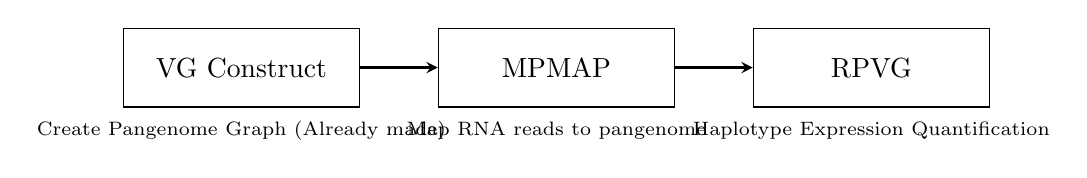
\begin{tikzpicture}[node distance=4cm]

  % Nodes
  \node (process1) [process] {VG Construct};
  \node (process2) [process, right of=process1] {MPMAP};
  \node (process3) [process, right of=process2] {RPVG};
 
% Notes (reduced space between nodes and notes)
\node[below of=process1, node distance=0.8cm, font=\scriptsize] {Create Pangenome Graph (Already made)};
\node[below of=process2, node distance=0.8cm, font=\scriptsize] {Map RNA reads to pangenome};
\node[below of=process3, node distance=0.8cm, font=\scriptsize] {Haplotype Expression Quantification};

  % Arrows
  \draw [arrow] (process1) -- (process2);
  \draw [arrow] (process2) -- (process3);
  
\end{tikzpicture}

\end{figure}

Pangenomes constructed were constrcuted by the VG Team, using samples from the 1000 Genomes 
Project.The same pangenomes and pantranscriptomes used in their paper were
used in this analysis, the pangenome used was created from all the european 
samples in the 1000 genomes database.\\

The VG Team published their Pangenomes and Pantranscriptomes on UC Santa Cruz's server

\url{http://cgl.gi.ucsc.edu/data/vgrna/pantranscriptomes/}\\

 
The VG Team as of writing this report has updated the format of their indexes for their 
pangenomes, thus an apptainer container, was built to run the older version of VG Tools.
Version 1.38.0 of VG Tools was used, as it was the same version used in the RPVG paper.\\

Example MPMAP command:

\begin{lstlisting}
  vg mpmap -n rna -t ${task.cpus} -x ${XG} -g ${GCSA} -d ${DIST} 
  -f ${R1} -f ${R2} > ${GAMP}
  \end{lstlisting}

  “.xg”: Spliced pangenome graph 

  “.gcsa”: GCSA index of pangenome graph 
 
  “.gcsa.lcp”: LCP array for gcsa
 
  “.dist”: Distance index of spliced pangenome graph 
 
  “.gbwt”: Pantranscriptome 
 
  “.gbwt.ri”: r-index of pantranscriptome 
 
  “.txt.gz”: Transcript and haplotype information

  "R1 and R2": Paired end RNA sequencing reads
  
  ".gamp": compressed allignment file\\

According to the VG Team, RPVG, does not work properly in a containerized environment, but
the team provided a pre compiled binary, which was used to run RPVG. Results from MPMAP are
fed into RPVG.\\

Example RPVG command:

\begin{lstlisting}
rpvg --use-allelic-mapq ${task.cpus} -g ${XG} -p ${GWBT} -a ${GAMP} 
-o ${OUTPUT} -i haplotype-transcripts -f ${TRANSCRIPT}
\end{lstlisting}

\section{Results}

\subsection{Accessing RPVG with Kallisto}

The VG Team published their ASE analysis, but only preformed their full analysis on one sample: NA12878

\url{https://zenodo.org/records/7234454}

Unlike standard ASE analysis, the VG team compared Transcripts per million (TPM) rather than counts per gene.
While unorthodox, other tools such as Kallisto output their results as TPM, although Kallisto is not
typically used for ASE analysis. RPVG produces results as either TPM or counts per transcript. Results 
from the VG team report were compared to synthesized data to assess the quality of their data. 
While their report compares RPVG to other popular RNA quantification tools (Kallisto, Salmon, RSEM),
they compare each tool against simulated data rather than against one another. 

To STARt this report, expands on the VG Team's comparision, by directly comparing the outputs of 
RPVG and Kallisto. Kallisto was chosen because it quantifies read counts on transcripts level like RPVG
and also produces results as TPM, to follow the same methods the VG team used. The same sample, NA12878,
from the same dataset from the RPVG paper was used in this comparison.

\begin{table}[H]
  \centering
  % First Table with Title
  \begin{minipage}{0.45\textwidth}
  \centering
  \textbf{RPVG} \\
  \vspace{0.25cm}
  \begin{tabular}{|l|r|}
  \hline
  \textbf{Statistic} & \textbf{Value} \\
  \hline
  count & \num{1.846557e8} \\
  mean  & \num{0.3622273} \\
  std   & \num{20.04858} \\
  min   & \num{0.000000} \\
  25\%   & \num{0.000000} \\
  50\%   & \num{0.000020748} \\
  75\%   & \num{0.000230361} \\
  max   & \num{21445.45} \\
  \hline
  \end{tabular}
  \end{minipage}%
  \hfill
  % Second Table with Title
  \begin{minipage}{0.45\textwidth}
  \centering
  \textbf{Kallisto} \\
  \vspace{0.25cm}
  \begin{tabular}{|l|r|}
  \hline
  \textbf{Statistic} & \textbf{Value} \\
  \hline
  count & \num{1.846557e8} \\
  mean  & \num{0.008625856} \\
  std   & \num{3.480867} \\
  min   & \num{0.000000} \\
  25\%   & \num{0.000000} \\
  50\%   & \num{0.000000} \\
  75\%   & \num{0.000000} \\
  max   & \num{17471.70} \\
  \hline
  \end{tabular}
  \end{minipage}
  \vspace{0.25cm}
  \caption{RPVG and Kallisto TPM Summary Statistics}  
\end{table}

Outputs of RPVG and Kallisto were compared, filtered for transcripts that mapped to both tools,
Table 1. RPVG produced a significantly higher mean TPM than Kallisto with, a 42-fold increase in average TPM. 
This matches the VG Team's claim that RPVG can map more reads, using a pangenome reference rather than a 
conventional fasta reference. While RPVG mapped more reads than Kallisto, this does not necessarily,
translate to higher quality data, as the standard deviation of 20 for RPVG. This is much higher than Kallisto's
standard deviation of ~3.5. RPVG produces results that are much more dispersed, than 
conventional methods.

\begin{figure}[H]
  \centering
  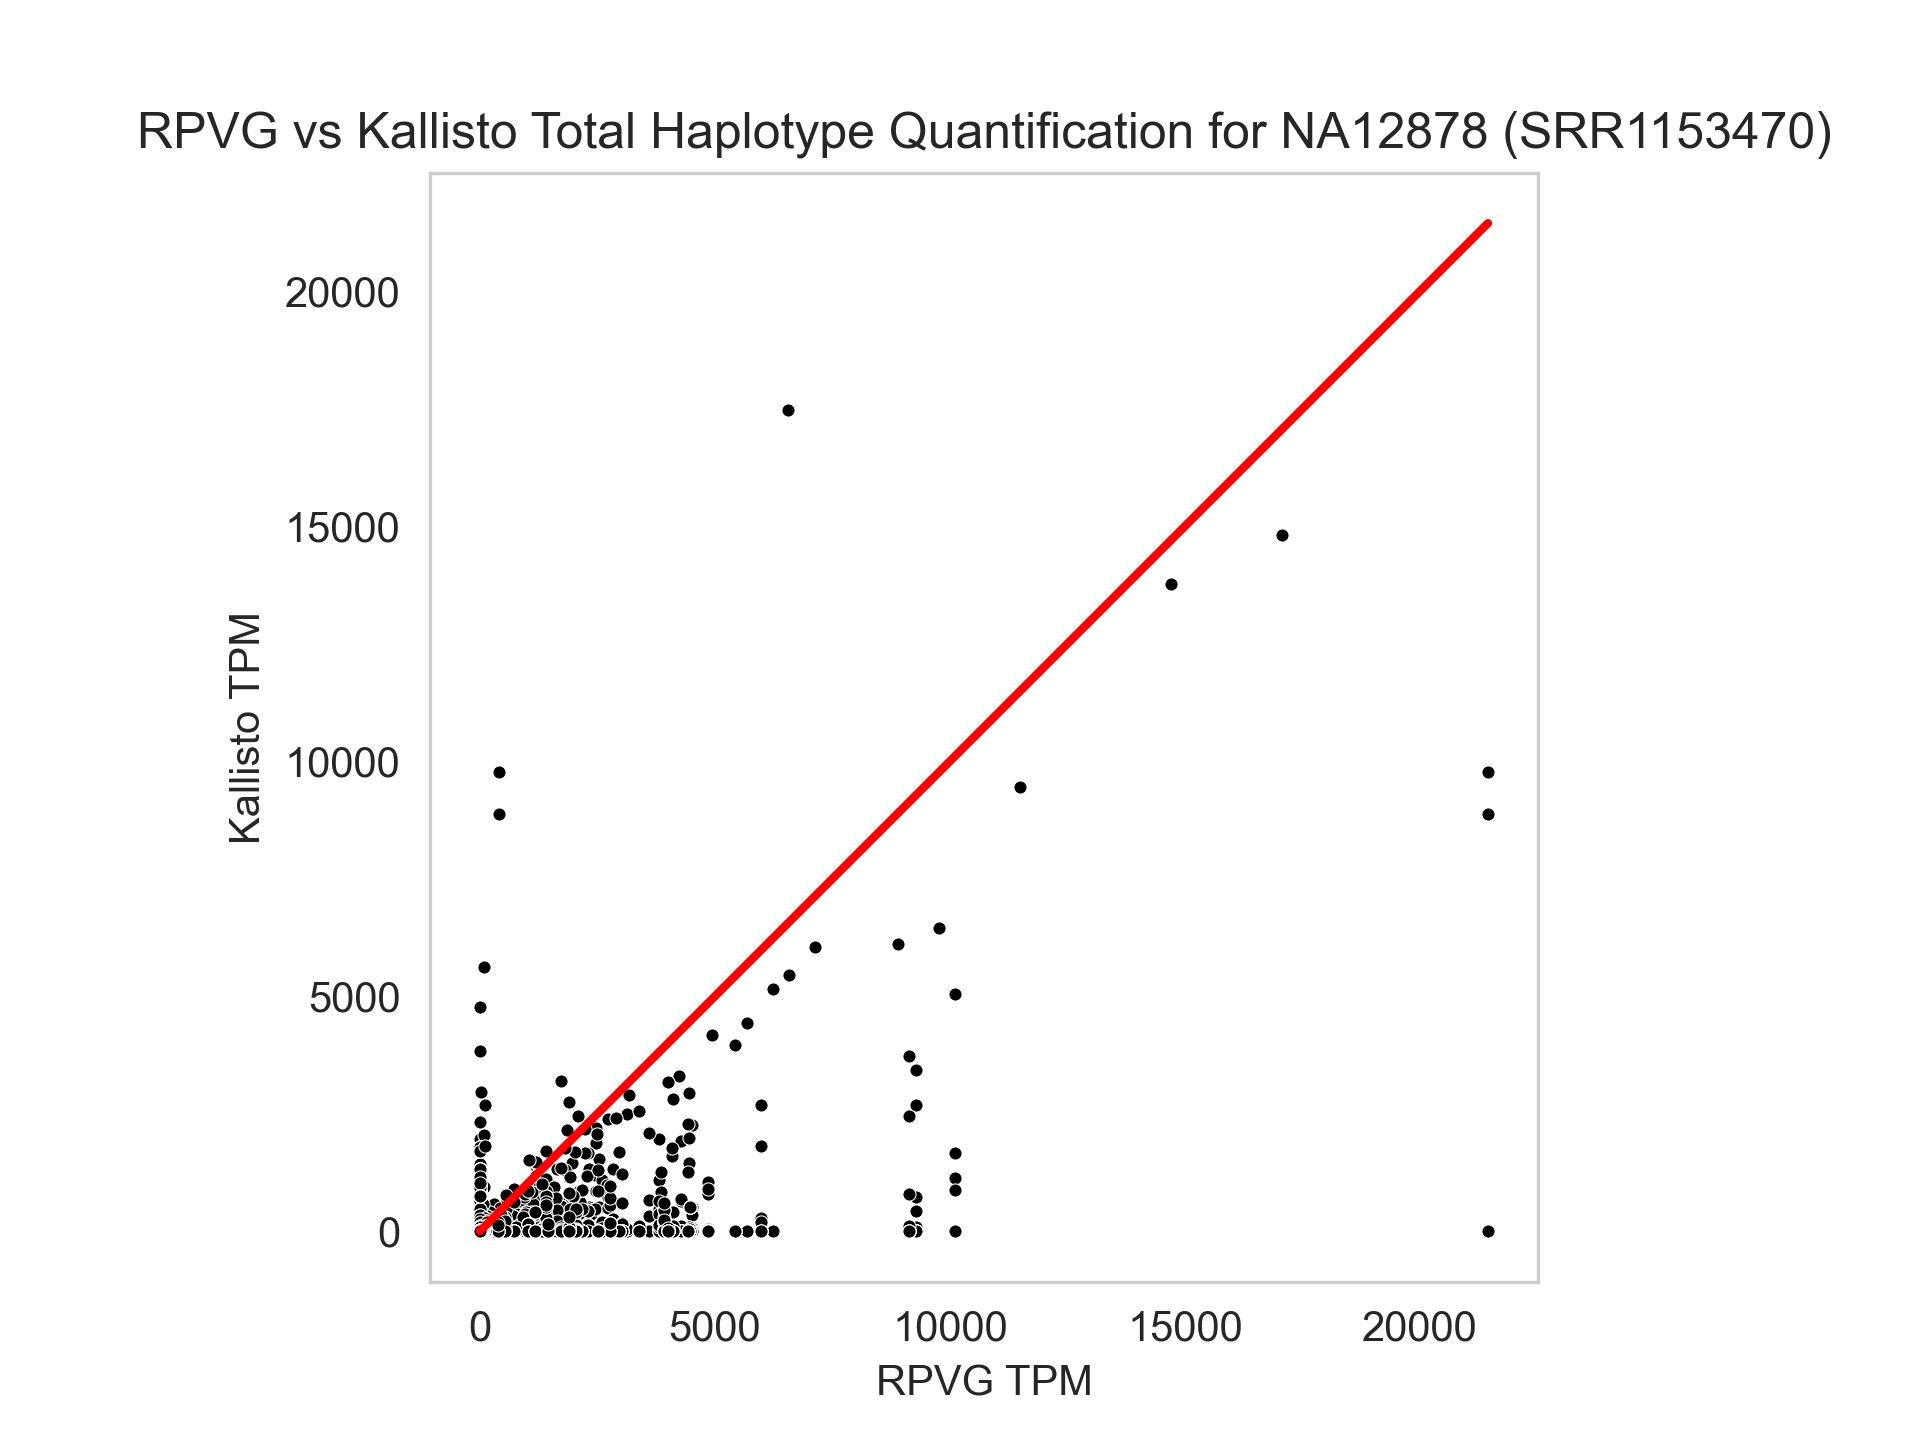
\includegraphics[width=0.8\linewidth]{Kallisto_vs_VG_Total_TPM.png}
  \caption{Kallisto and RPVG Transcripts Per Million (TPM) for NA12878, the sample used in the paper. A line with a slope of 1 shows
  where TPM for both methods are equal. A filter to remove transcripts with less than 50 TPM for where total haplotype 
  count was less than 50, was applied to make visualization more clear.}
\end{figure}

\vspace{5em} % Add vertical space here

Figure 2 shows that while RPVG mapped more reads for the majority of transcripts, compared to
the output of Kallisto, the increased number of read counts per transcript, is not consistently increasing. 
Some transcripts are more expressed than others relative to the results from Kallisto. A more 
the linear trend would be expected if RPVG was producing better 
results than Kallisto, with all transcripts showing a similar increase in counts.
RVPG was able to map many more transcripts than Kallisto, which may be in part due to using
a Pangenome reference which is more inclusive than a standard reference. RPVG also has a 
more lenient mapping algorithm, as RPVG maps partial transcripts, and includes it in the read count. 

\begin{figure}[H]
  \centering
  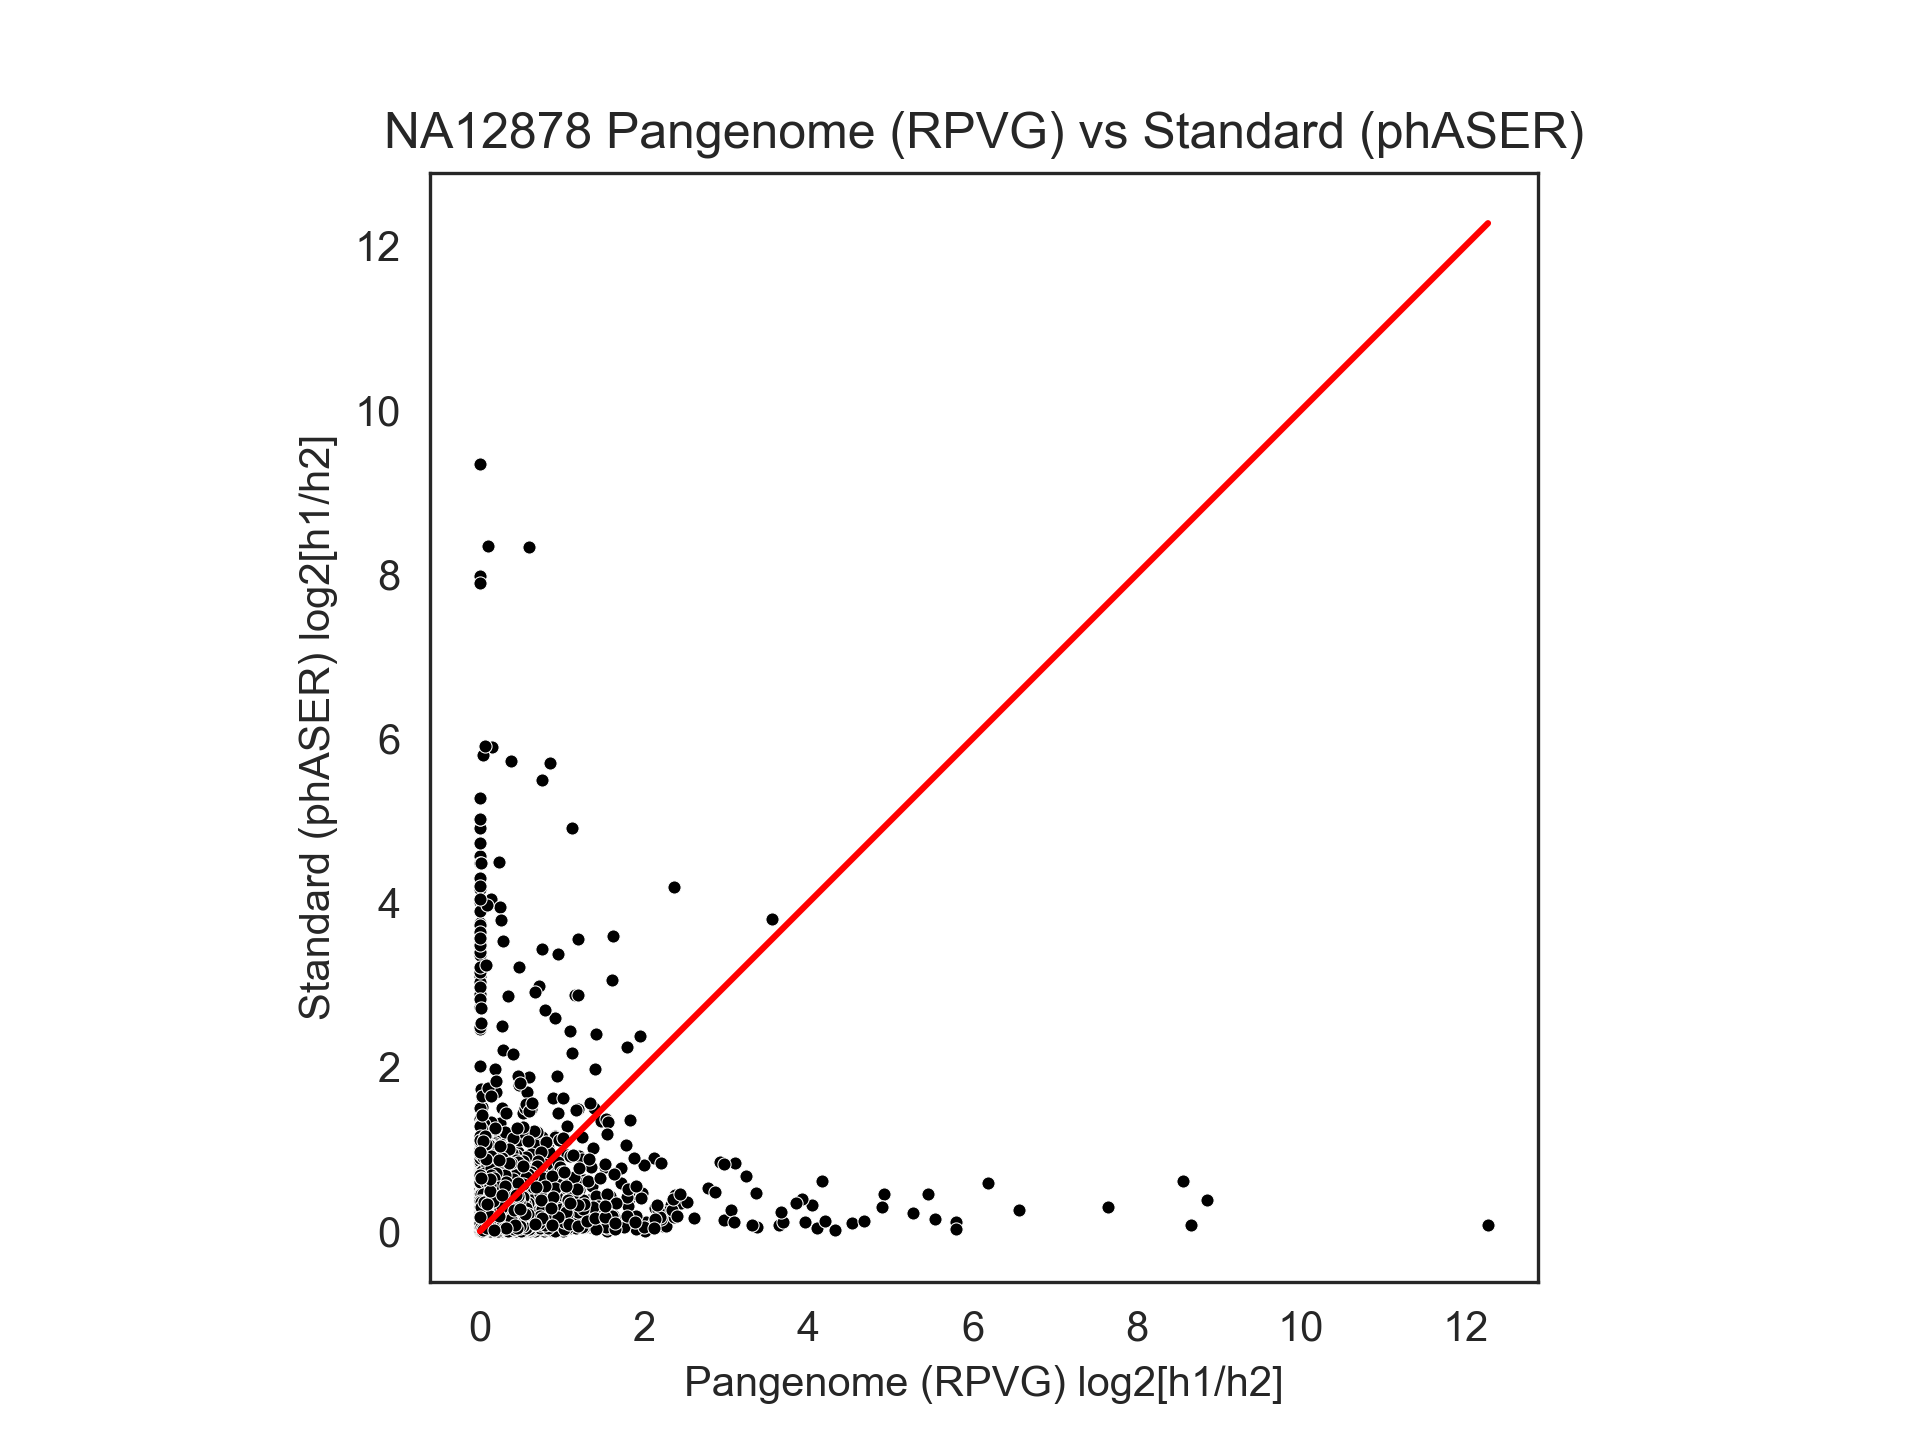
\includegraphics[width=0.8\linewidth]{NA12878_Pangenome_vs_Standard_log_Filter_50.png}
  \caption{Pangenome (RPVG) vs Standard (phASER) log 2 [Hap 1/ Hap 2] for NA12878. A filter to remove total gene counts of less than 50, was applied to make visualization more clear.
  } 
\end{figure}  

RPVG was compared against, standard ASE data generation methods 
(Alignment with STAR \citep{Dobin_2012}, counting and read counting done with phASER \citep{Castel_2016}). The comparison
was done by taking the natural log of the ratio of haplotype 1 divided by haplotype 2, for each gene, for RPVG
and Standard ASE methods for the same sample. This allowed a comparison of the level of expression of 
each haplotype from both methods. Figure 3 shows no clear linear relationship between the two methods,
while RPVG and MPMAP may produce more counts, it is not able to consistently discern which, genes are 
overexpressed, a somewhat linear relationship would be expected if RPVG could properly determine the same
level of expression as standard methods.

In order to compare RPVG results which are on a transcript level, to standard ASE analysis methods, RPVG results needed to be 
converted to gene level. This was done by mapping back RPVG transcript outputs back to the original 
annotation file which contained a key of genes and transcripts. 
Transcrips were summed, for genes that contained multiple transcripts. The comparison of 
RPVG and Standard methods were done with counts per gene.

\subsection{Accessing RPVG with MAGE dataset}

MAGE is a diverse, high-quality dataset with samples resequenced from the 1000 Genomes 
Project. \citep{Taylor_2024} If results from RPVG were promising, this dataset contains samples from
all over the world, and the pangenome analysis would be run on the entire dataset. 

20 Samples from the MAGE Dataset were run through MPMAP and RPVG and compared against, 
ASE data generated from standard ASE methods. The standard ASE data had been previously QCed and is a high-quality reference
to see where ASE data produced by RPVG differs. These 20 samples run through RPVG, did not produce
clean ASE data, and to save computational resources the rest of the MAGE dataset was not run through 
the HPC cluster. One sample, HG00114 is shown here for the rest of the graphs, as all other samples,
produced similar results, however, the figures for all samples are available in the supplemental materials.

Because RPVG produced counts on a transcript level, RPVG datasets 
were remapped back to gene level to be compared to the phASER output
which was also on gene level.

%\vspace{-10pt}
\begin{figure}[htbp]
  \centering
  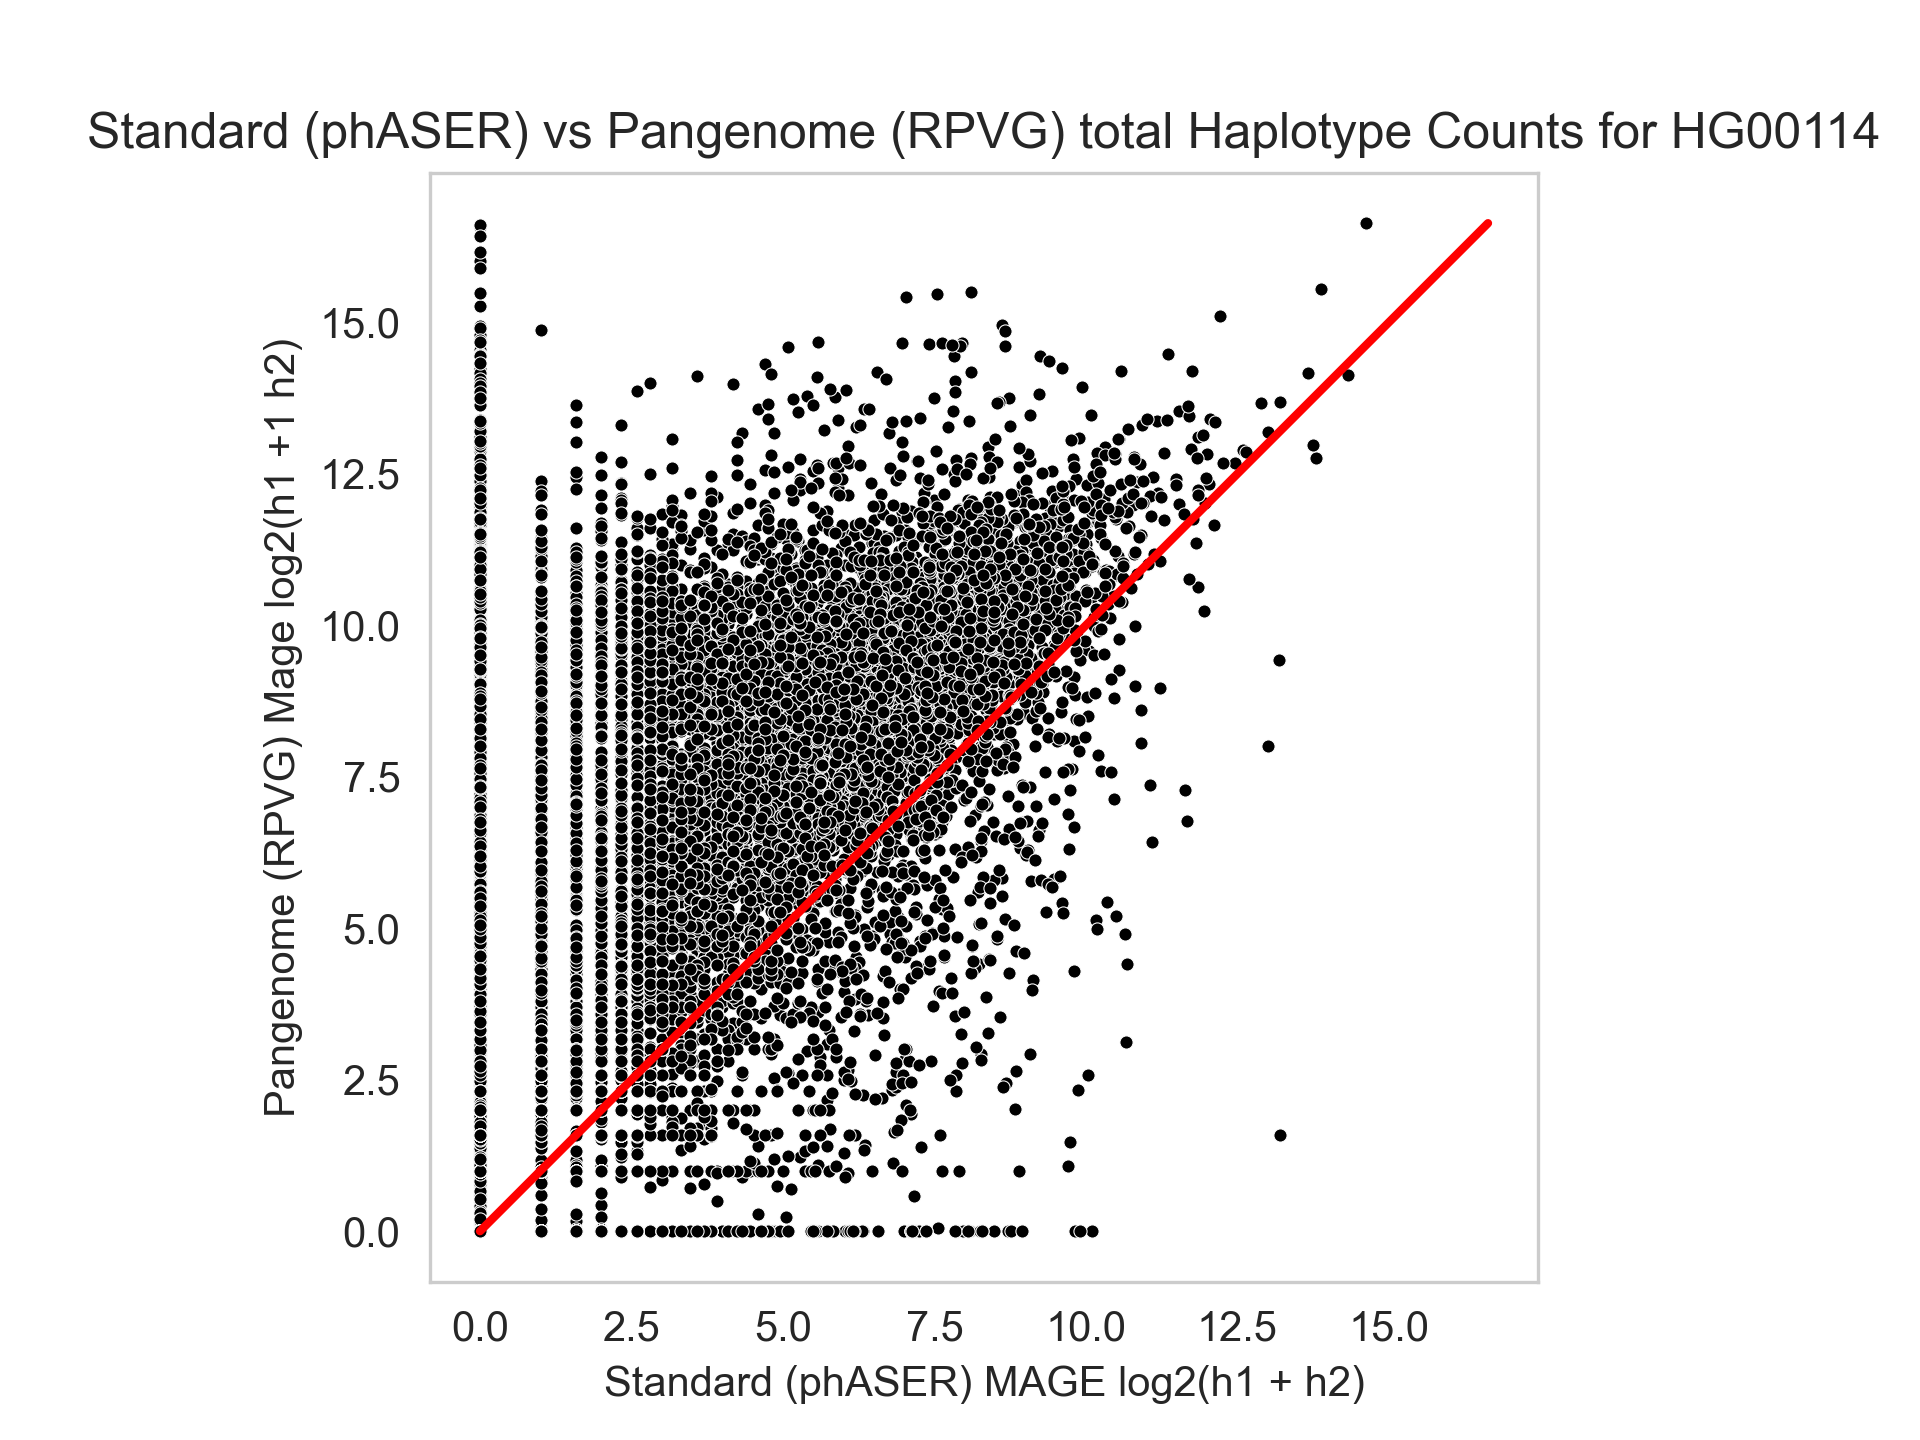
\includegraphics[width=0.8\linewidth]{HG00114_PAN_MAGE_log_plot.png}
  \caption{Pangenome (RPVG) vs Standard (phASER) Total counts for HG00114. A line with a slope of 1 shows
  where total counts for both methods are equal.}
\end{figure}  
\vspace{2em}

When running the RPVG pipeline on the MAGE dataset, RPVG and MPMAP produced significantly more counts 
than MAGE data generated with STAR and phASER. RPVG produced more counts for almost all genes 
compared to standard ASE methods. Banding patterns between 0 and 2 for the standard ASE data, are 
regions of the genome that are masked, and not counted, as they are repetative regions of the genome.
These regions are difficult to align properly using traditional methods and are usually not counted.

%\vspace{-8pt}
\begin{figure}[htbp]
  \centering
  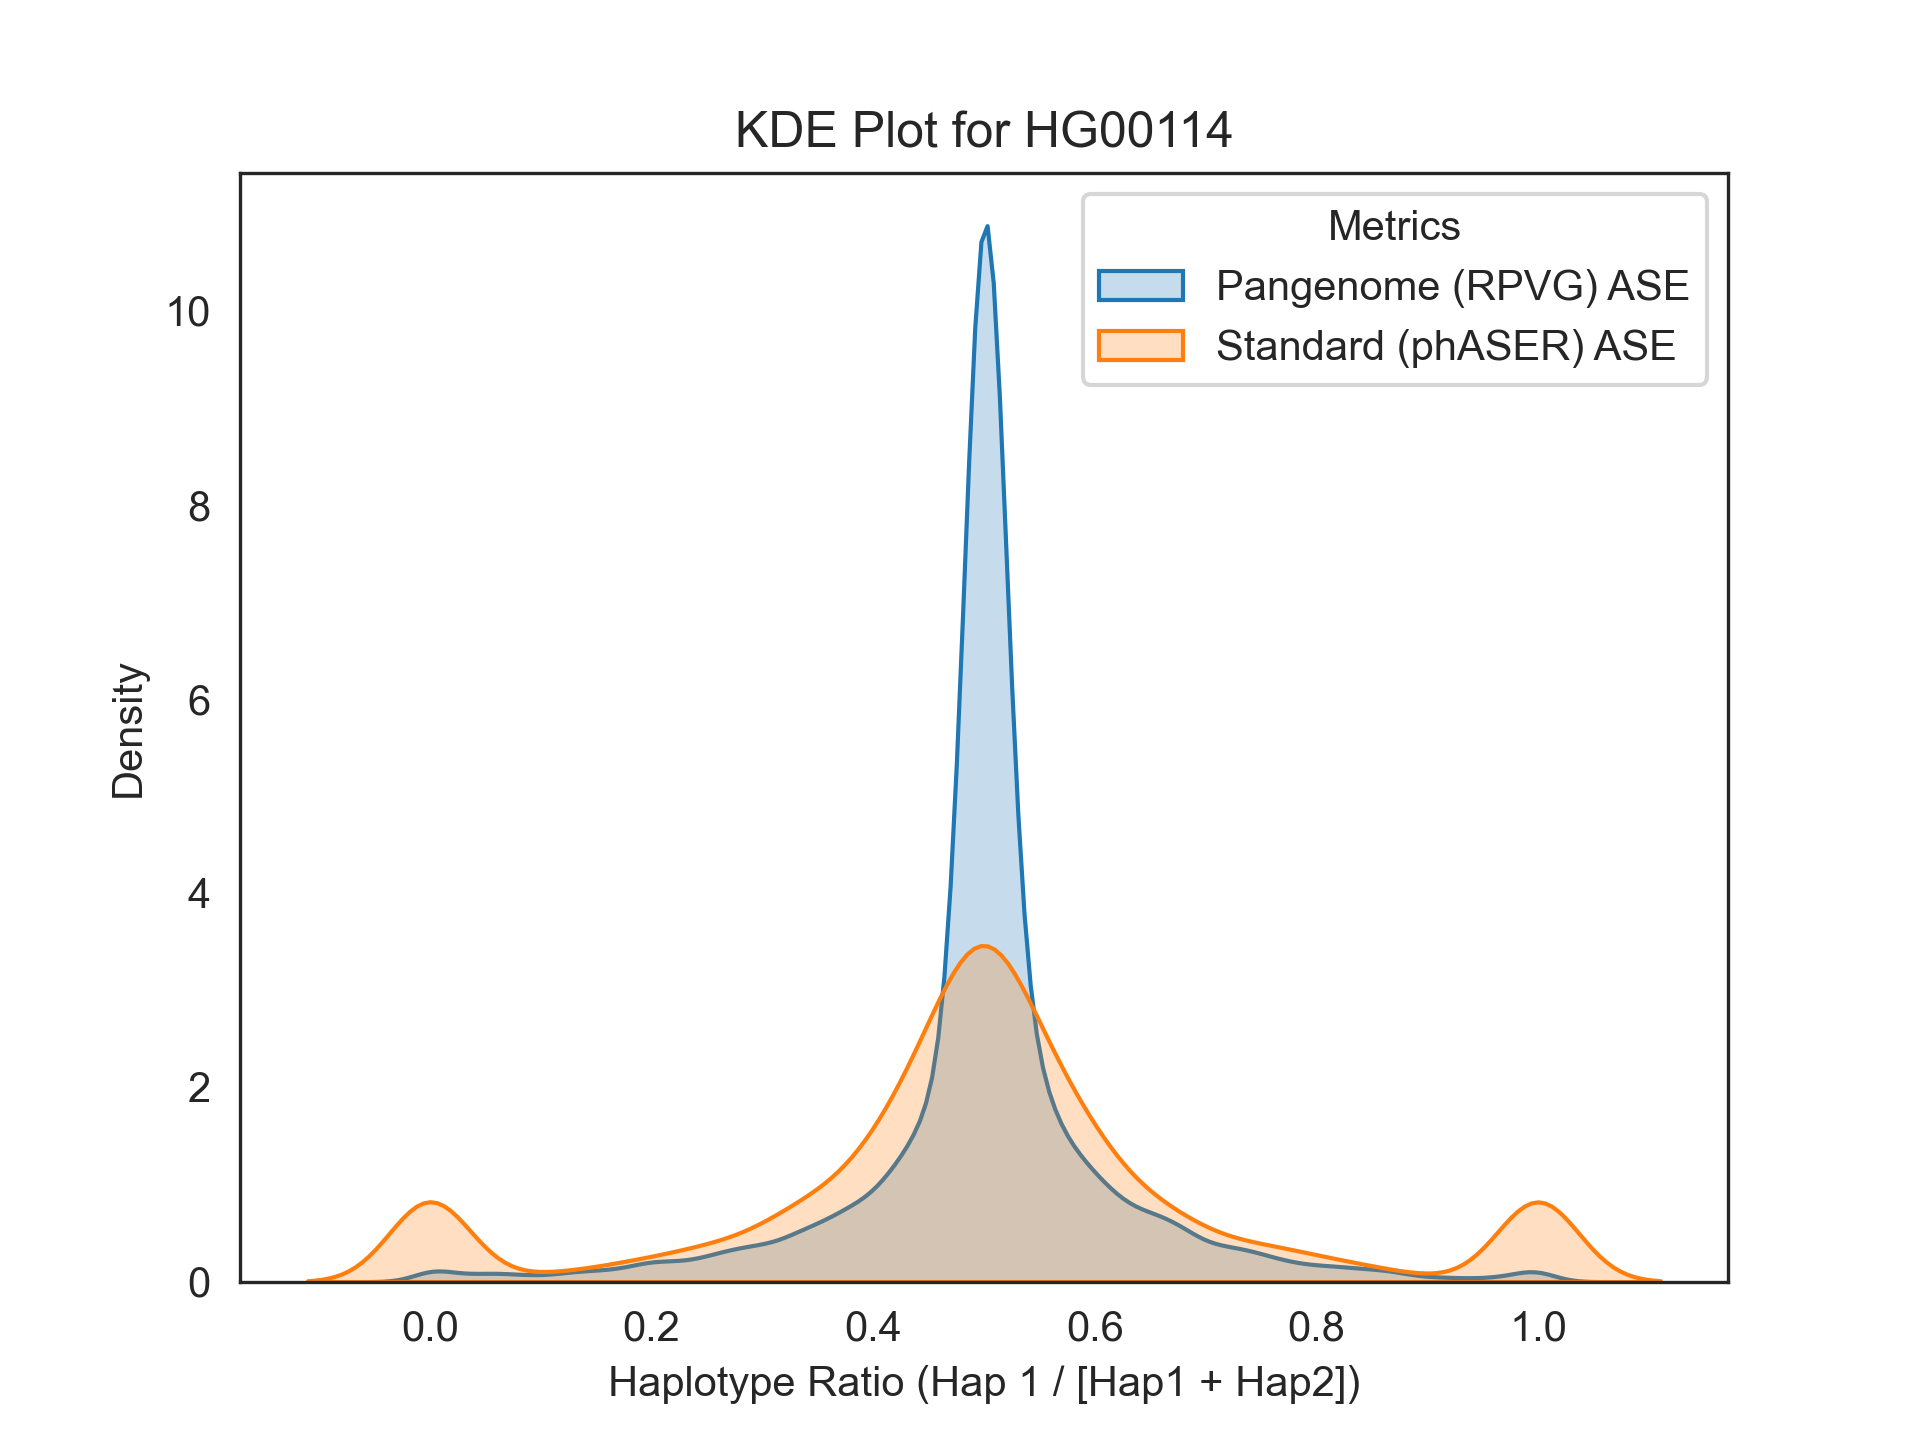
\includegraphics[width=0.8\linewidth]{HG00114_PAN_MAGE_kdeplot.png}
  \caption{Kernel density estimate (KDE) to show density of haplotype expression ratio of two 
  haplotypes. Haplotype 1 / Total Counts for Pangenome (RPVG, Blue) and Standard (phASER, Orange) total counts for HG00114.}
\end{figure}  
%\vspace{-10pt}

A KDE plot of both datasets shows that the majority of the dispersion for both plots is 
around 0.5, which is expected as most genes should not be overexpressed. Figure 5, RPVG (Blue) had a much higher peak at
the 0.5 mark, compared to phASER (RED), which was more dispersed around 0.5 when comparing expression levels of 
haplotype 1 divided by total haplotype expressed (haplotype 1 + haplotype 2). In the output files from RPVG,
there were many points where both haplotypes had the same counts. This is surprising as
RPVG already produced counts that contained fractional outputs. For the majority of genes
to have an exact ratio of 0.5, compaired to phASER, which produces outputs as whole numbers and with a 
more natural dispersion around 0.5, is unlikely. It appears RPVG is estimating the haplotype ratios for these genes.

\subsection{ASE analysis of results}

\begin{figure}[H]
  \centering
  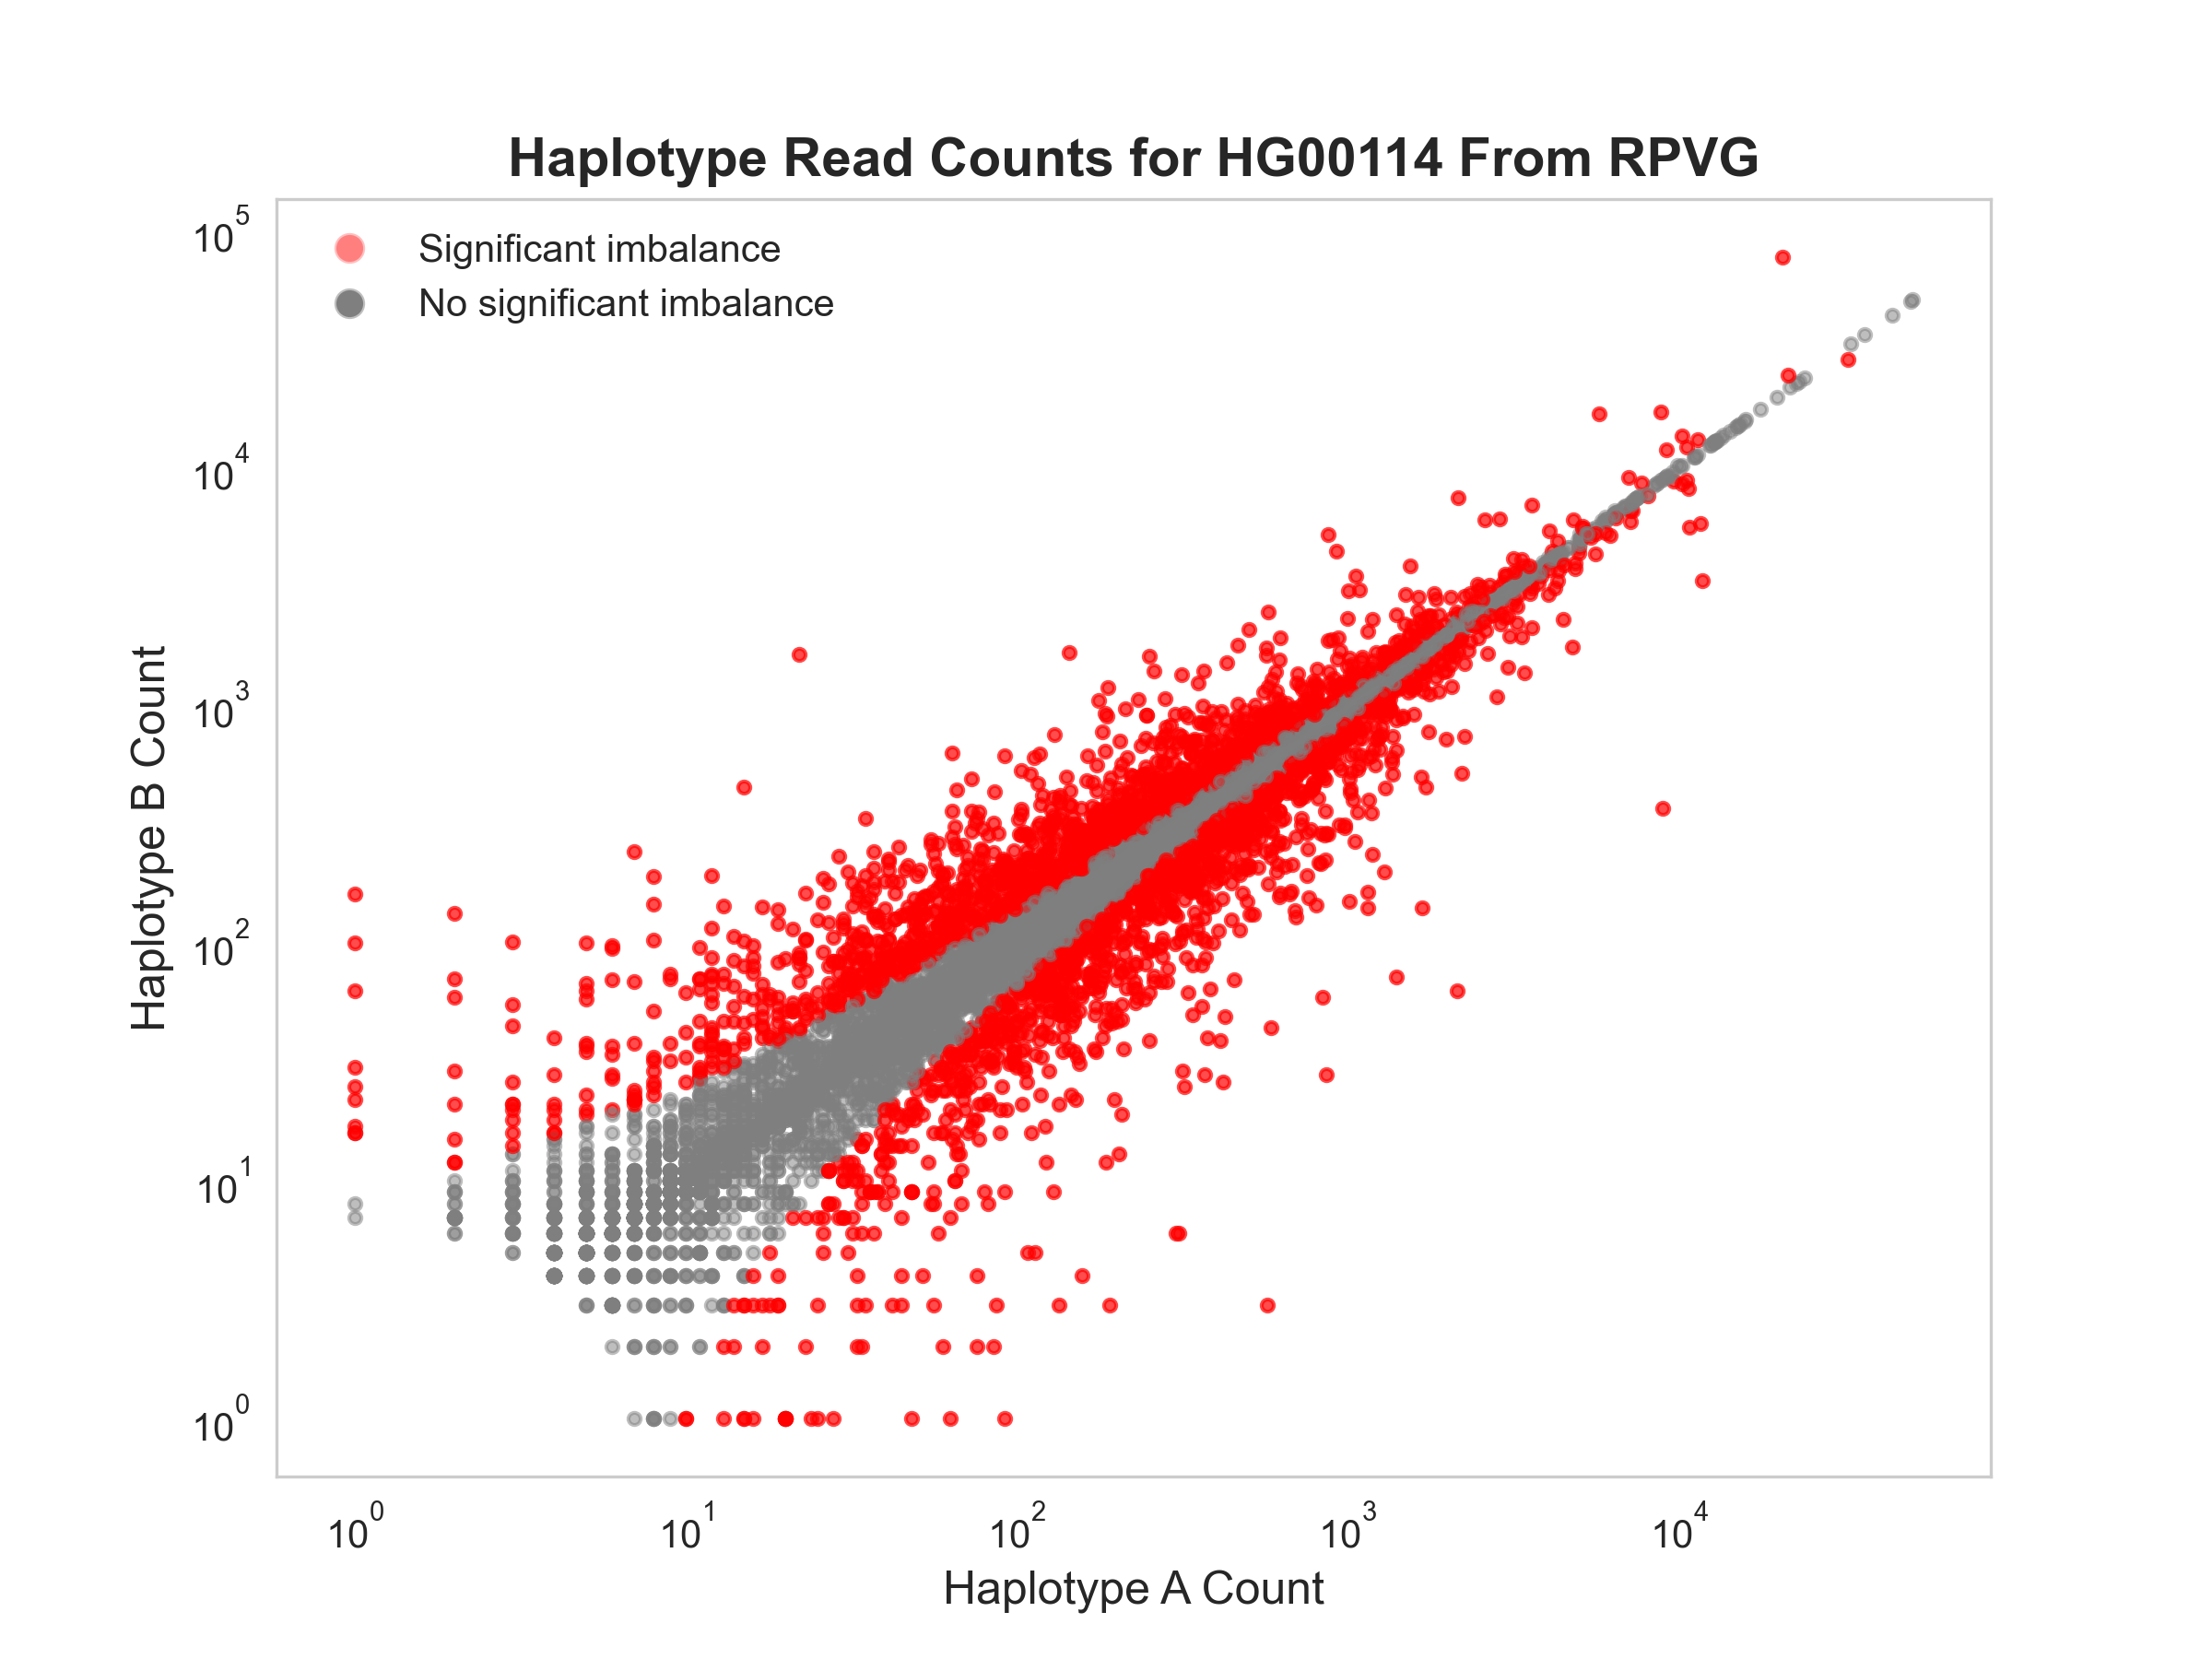
\includegraphics[width=0.8\linewidth]{HG00114_RPVG.png}
  \caption{Comparision of haplotype expression with a binomial distribution for 
  HG00114, produced with RPVG.}
\end{figure}  

\begin{figure}[H]
  \centering
  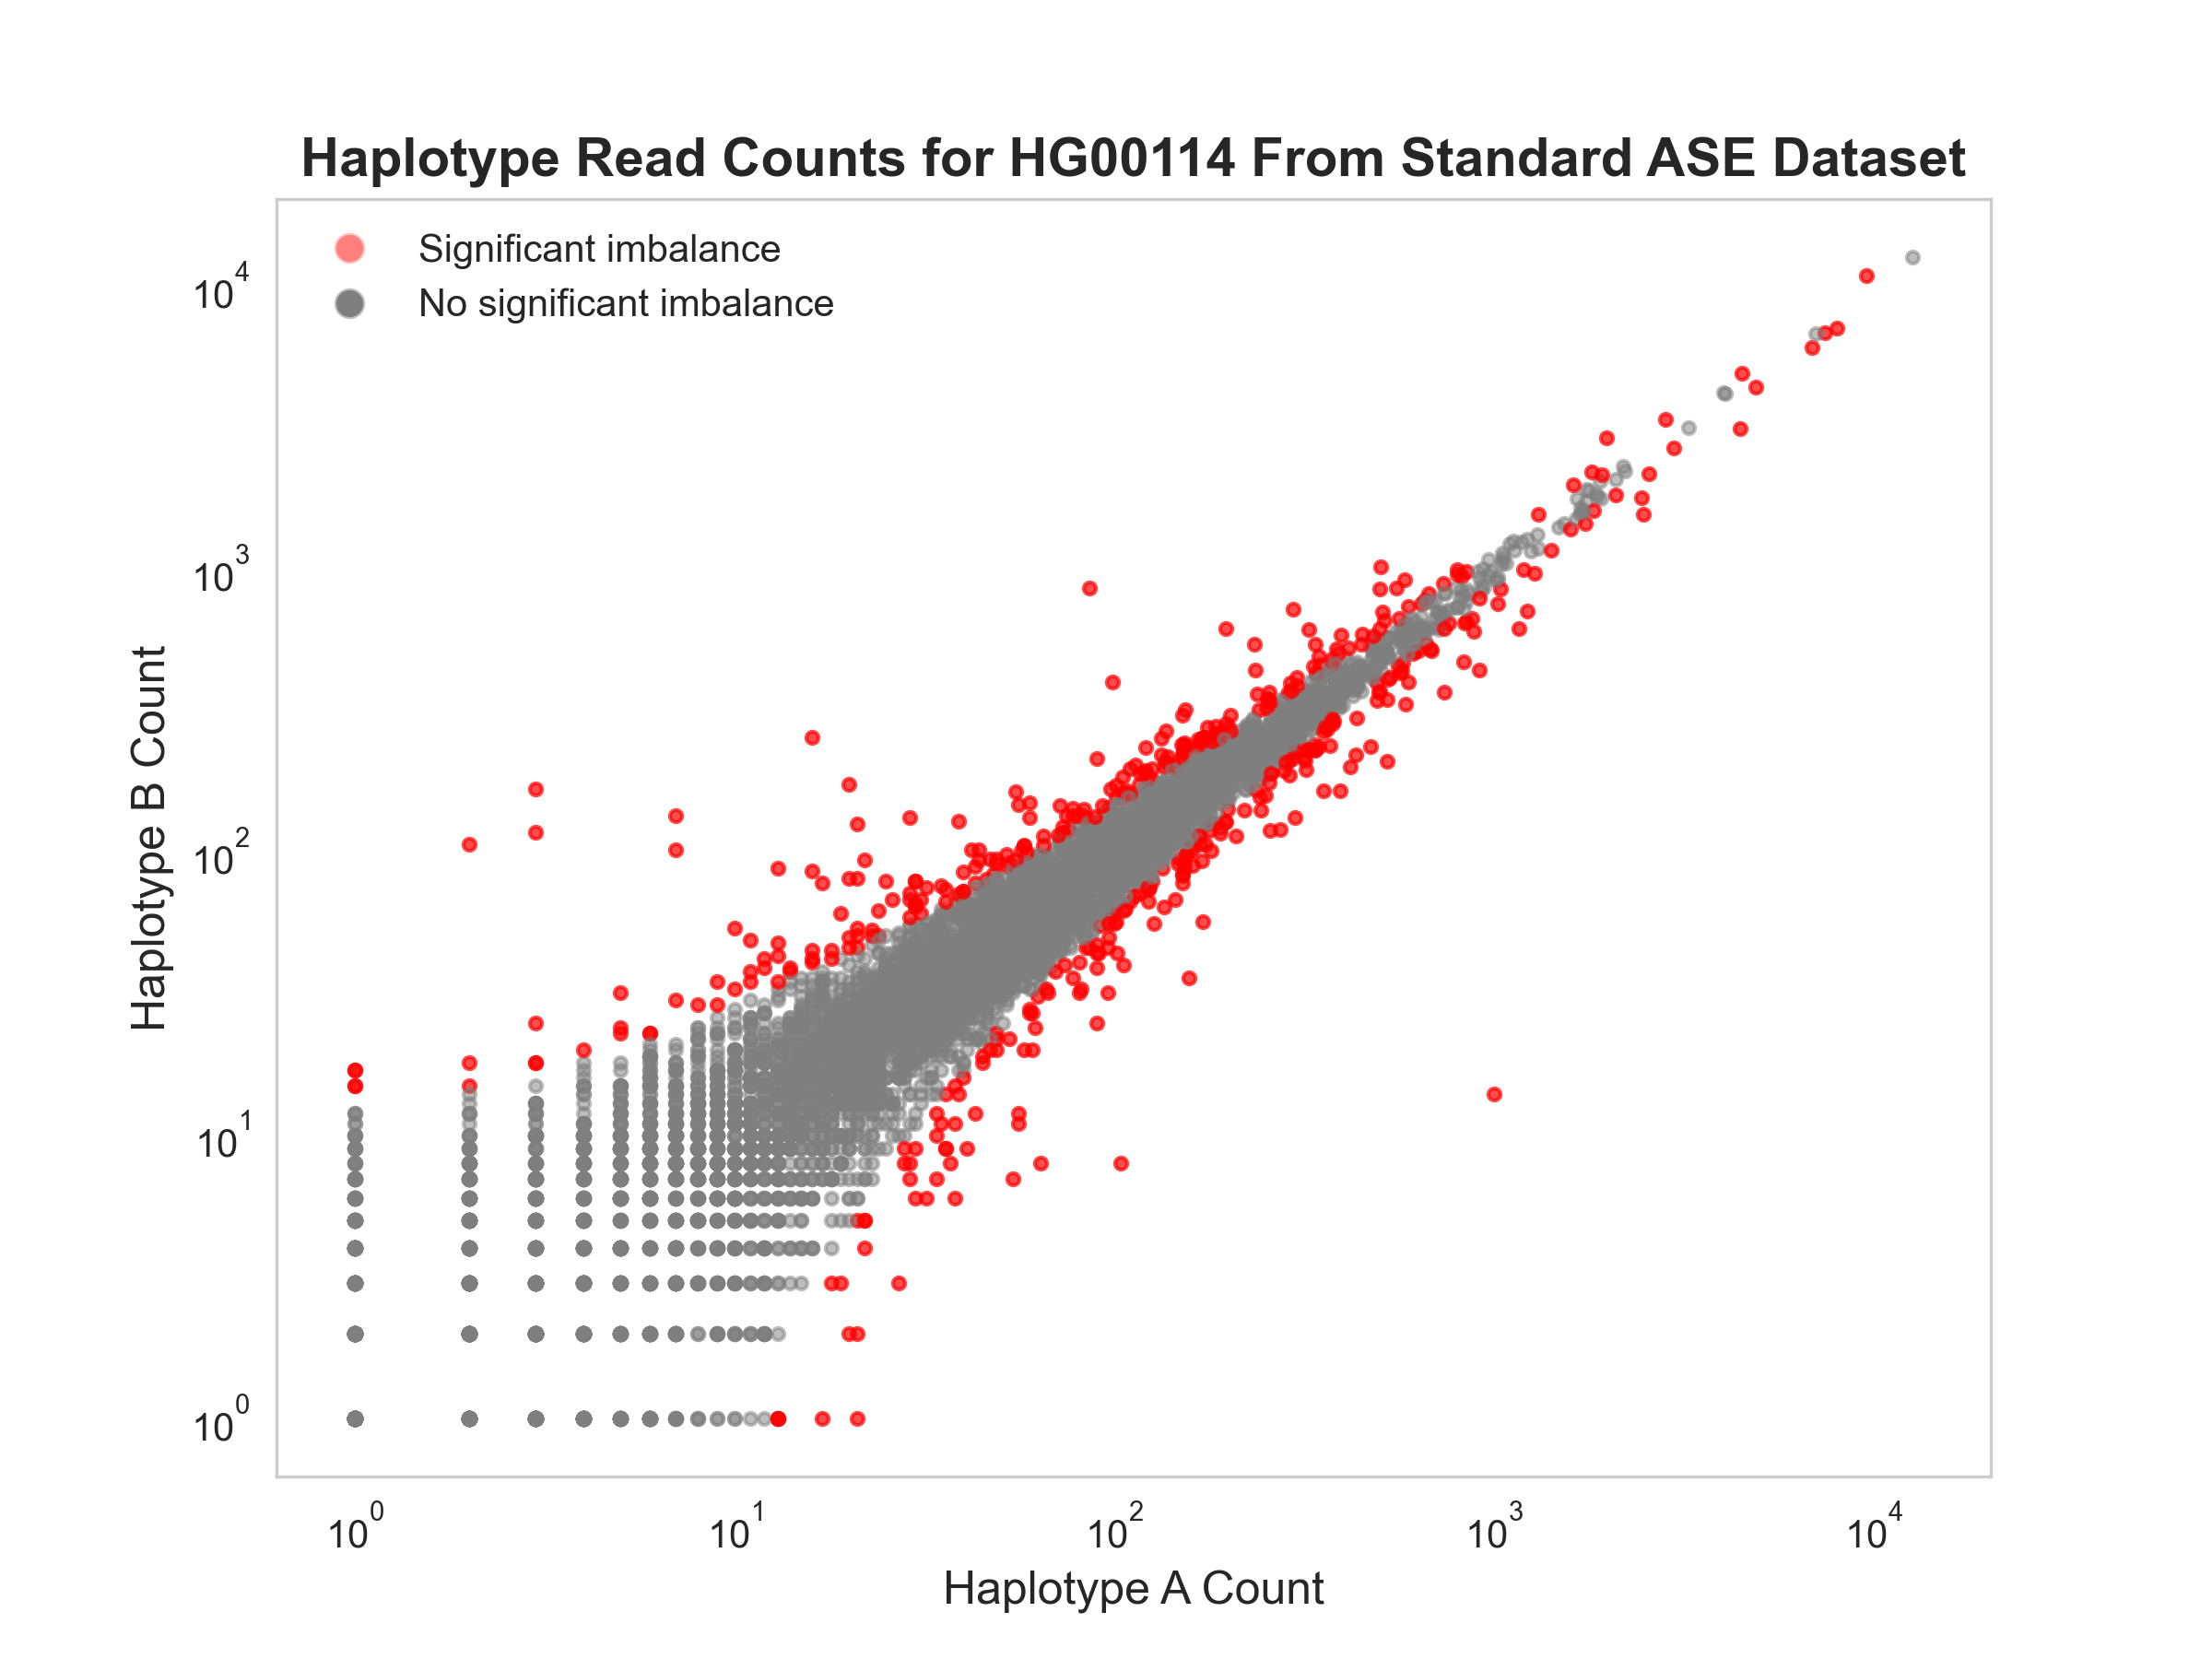
\includegraphics[width=0.8\linewidth]{HG00114_Standard.png}
  \caption{Comparision of haplotype expression with a binomial distribution for 
  HG00114, produced with standard tools (phASER).}
\end{figure}  

A binomial test was performed on the output of RPVG against the standard ASE analysis output from phASER, 
to measure the expression of each haplotype
with points considered as overexpressed and outside of a 95 percent confidence interval highlighted 
in red. Figure 7 shows haplotype expression for data generated from standard methods and is an example
of what standard ASE output generally looks like. Most genes are not expected to be overexpressed, and 
with most points falling along a linear trend, of a slope of 1, where expression levels are almost equal. 

Figure 6 shows the output of RPVG, not only are more genes overexpressed, but the level of expression
is much higher generally than the standard ASE data for the same sample. There is a lot more noise
or dispersion in RPVG data, making it difficult to determine which genes are truly overexpressed.

\section{Discussion}

While RPVG is a promising tool, producing more counts does not necessarily 
translate to higher-quality data. Although RPVG produced significantly
more counts than Kallisto or phASER in this analysis, as well as with other tools in the 
RPVG paper, further analysis told a different story.

ASE data produced by RPVG was significantly overexpressed, for all samples
after a binomial test was performed. If the results of RPVG were taken at
face value, this would suggest that all previous ASE analyses were done
incorrectly and that more alleles than expected are expressed, and the level of expression
for those genes would be much higher. 

Furthermore, RPVG failed to reproduce QCed
high-quality ASE data from a dataset generated using standard tools and methods. While
it was expected that RPVG would not match the results of previous tools exactly 
and that there would be more counts for some genes, to produce such highly different results
suggests that RPVG is not producing accurate reproducible results. RPVG also produced a large
number of genes with exact same levels of expression, even though the output of RPVG contains fractional
counts. This suggests that RPVG is trying to predict counts for a given transcript, but 
is unable to infer the other haplotype properly.

RPVG functions very differently than other tools, with similar functions
as a genotype is not used for ASE analysis, and that RPVG predicts possible transcript 
paths based on how the reads map to the pangenome reference. 

The additional counts produced by RPVG were likely due to a few factors. Using a graph 
reference with the pangenome
alignment of RNA reads in MPMAP and later in the pantranscriptome, with RPVG likely mapped
more reads that other tools were unable to, this is in part by design. The mapping
algorithm however was likely too lenient, in the step where they allowed partial alignments to a 
transcript. This is also likely why their output for RPVG does not produce whole numbers for
read counts, including fractional counts instead. Furthermore counting on a transcript level
makes it difficult to compare to previous ASE analyses, which are commonly done on gene level. The 
conversion of the transcript to gene likely compounded the already high counts. 

If the VG Team
were to improve their tool, adding an option to produce counts on a gene level, would be 
beneficial for future studies. The VG team are very experienced in the field of Pangenomics,
this is their first paper discussing ASE analysis and in the future, if they want to improve
RPVG, working with experts in the field of ASE analysis is essential.

These results in this project were overlooked by the VG team, as they only analyzed one sample for ASE, and 
did not perform a proper ASE analysis. Instead, they compared their results to expected
simulated results. It is unfortunate, that in its current state, RPVG, does not produce
reproducible results as there is a lot of potential in the tool, and in using graph references for ASE 
analysis as a whole. 
Running MPMAP and RPVG is a much more straightforward process to produce ASE data, compared to standard methods
using STAR, andASEReadCounter or phASER. With standard methods, input options need to be 
catered to each sample, and for haplotype analysis, results must be phased. 
RPVG, also may work better by aligning to repetitive regions of the human genome
that are currently have to be masked with traditional ASE methods, as
graph references may make alignments easier to these regions of the genome. 
RPVG is currently the only tool that can use Pangenome graphs as input for ASE analysis, and
until RPVG is improved, or a new tool comes along, the issue of reference bias will need
another solution.

\vspace{35em}

\section{Supplemental Materials}

All code use the pipeline and used are figures are available on github.
Additional figures for the rest of the MAGE dataset, are also available on the github: \\
\url{https://github.com/Cave42/Pangenome_ASE}

\begin{table}[H]
  \centering
  \renewcommand{\arraystretch}{1.3} % Increase row height
  \setlength{\tabcolsep}{10pt} % Adjust column spacing
  \begin{tabular}{|c|c|}
      \hline
      \textbf{Sample ID} & \textbf{SRR ID} \\ \hline
      HG00265 & SRR19762408 \\ 
      HG00260 & SRR19762234 \\ 
      HG00254 & SRR19762504 \\ 
      HG00250 & SRR19762660 \\ 
      HG00244 & SRR19762665 \\ 
      HG00243 & SRR19762419 \\ 
      HG00237 & SRR19762247 \\ 
      HG00233 & SRR19762678 \\ 
      HG00160 & SRR19762584 \\ 
      HG00151 & SRR19762718 \\ 
      HG00148 & SRR19762787 \\ 
      HG00146 & SRR19762594 \\ 
      HG00142 & SRR19762732 \\ 
      HG00141 & SRR19762808 \\ 
      HG00132 & SRR19762855 \\ 
      HG00130 & SRR19762612 \\ 
      HG00127 & SRR19762815 \\ 
      HG00122 & SRR19762869 \\ 
      HG00121 & SRR19762757 \\ 
      HG00114 & SRR19762921 \\ \hline
  \end{tabular}
  \vspace{0.25cm}
  \caption{MAGE Dataset Samples Selected, run and analysised for this project}
  \label{tab:sample_data}
\end{table}


\bibliographystyle{plainnat}
\bibliography{references}

\end{document}